\documentclass[9pt,aspectratio=169]{beamer}
\usepackage[T2A]{fontenc}
\usepackage[utf8]{inputenc}
\usepackage[english,russian]{babel}
\usepackage{color} 
\usepackage{wrapfig}
\parindent=0.7cm
\usepackage{graphicx}

\defbeamertemplate*{frametitle}{shadow theme}{
	\color[rgb]{0.65,0.65,0.65}
	\begin{flushright}
		\textbf{\insertframetitle}
	\end{flushright}
	\hline
	\vskip -1cm\hskip -0.8cm
\includegraphics[scale=0.4]{beamerlogo.png}
}

\begin{document}
	\begin{frame}{Анализ свойств меры Хартли}
		\noindent Экспериментатор одновременно подбрасывает монету (М) и кидает игральную кость (К).
		Какое количество информации содержится в эксперименте (Э)?\\
		\vspace{1.5em}
		\color[rgb]{0.2,0.7,0.4}
		\noindent\textbf{Аддитивность:}\\
		\color{black}
		$i(\mbox{Э})=i(M)+i(K)=>i(\mbox{12 исходов})=i(\mbox{2 исхода})+i(\mbox{6 исходов}):\ \log_x12=\log_x2+\log_x6$\\
		\color[rgb]{0.2,0.7,0.4}
		\noindent\textbf{Неотрицательность:}\\
		\color{black}
		Функция $log_xN$ неотрицательно при любом $x>1$ и $N\geq1$\\
		\color[rgb]{0.2,0.7,0.4}
		\noindent\textbf{Монотонность:}\\
		\color{black}
		С увеличением $p(M)$ или $p(K)$ функция $i(\mbox{Э})$ монотонно возрастает.\\
		\color[rgb]{0.2,0.7,0.4}
		\noindent\textbf{Принцип неопределённости:}\\
		\color{black}
		При наличии всегда только одного исхода (монета и кость с магнитом) количество\\
		информации равно нулю: $\log_x1+log_x1=0$
	\end{frame}
	\begin{frame}{Мера количества информации по Шеннону}
	    \begin{wrapfigure}[3]{r}{0.2\textwidth}
	        \begin{center}
	            \vskip -1cm
   				 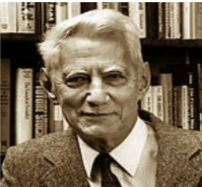
\includegraphics[width=0.20\textwidth]{17}
  			Клод Шенном\\ (1916-2001)
  			\end{center}
    	\end{wrapfigure}
		\noindent Мера Хартли подходит лишь для систем с равновероятными состояниями. 
		\noindent Если состояния системы S не равновероятны, используют меру Шеннона:
		$$i(S)=-\sum_{i=1}^Np_i\cdot log_2p_i,$$
		где N – число состояний системы,\\
		\noindent рi – вероятность того, что система S находится в\\
		\noindent состоянии i (сумма всех $p_i$ равна 1).
		\vspace{0.2cm}
		\begin{center}
			\color[rgb]{0.2,0.7,0.4}
			\textbf{Формула Хартли является частным случаем формулы Шеннона!}
			\color{black}
		\end{center}
		\noindent\textbf{Пример 1.} Количество информации в акте подбрасывания обычной монеты по формуле Хартли равно $\log_22=1$ бит. По 				формуле Шеннона получим то же $i_{s1}=-0,5*\log_20,5-0,5*\log_20,5=1$ бит.\\
		\noindent\textbf{Пример 2.} При подбрасывании монеты со смещённым центром тяжести количество непредсказуемости становится меньше: 				$i_{s2}=-0,75*\log_20,75-0,25*\log_20,25\approx0,8$ бит.
	\end{frame}
	\begin{frame}{Пример использования меры Шеннона}
	    \vspace*{-20mm}
	    \noindentШулер наугад вытаскивает одну карту из стопки, содержащей 9 известных ему карт: 3\\
        \noindentджокера, 3 туза, 1 король, 1 дама и 1 валет. Какое количество информации для шулера\\
        \noindentсодержится в этом событии s?
        
        Вероятность вытащить: $\left\{
        \begin{array}{l}
             \mbox{джокера}\\
             \mbox{туза}\\
             \mbox{короля}\\
             \mbox{даму}\\
             \mbox{валета}
        \end{array}\right\}$ равна $\left\{
        \begin{array}{l}
             \mbox{3/9 = 1/3}\\
             \mbox{3/9 = 1/3}\\
             \mbox{1/9}\\
             \mbox{1/9}\\
             \mbox{1/9}
        \end{array}
        \right .$ \\
        \begin{center}
        
        $i(s) = -(\frac{1}{3}*\log_3{\frac{1}{3}} + \frac{1}{3}*\log_3{\frac{1}{3}} + \frac{1}{9}*\log_3{\frac{1}{9}} + \frac{1}{9}*\log_3{\frac{1}{9}} + \frac{1}{9}*\log_3{\frac{1}{9}}) = $\\
        $\frac{1}{3} + \frac{1}{3} + \frac{2}{9} + \frac{2}{9} + \frac{2}{9} = 1\frac{1}{3}$ $\approx$ $\log_3{5}$ vs $\log_3{14}$ 
        \end{center} 
	\end{frame}
	\begin{frame}{Нестрогий вывод формулы Шеннона}
	        \vspace*{-10mm}
	        \color[rgb]{0.2,0.7,0.4}
			\noindent Задача.
			\color{black}
	        Монета имеет смещённый центр тяжести. Вероятность выпадения «орла» – 0,25,\\
            вероятность выпадения «решки» – 0,75. Какое количество информации содержится в одном\\
            подбрасывании?\\
            
            \color[rgb]{0.2,0.7,0.4}
			\noindent Решение
			\color{black}
	        \begin{itemize}
	            \item[\textbullet] Пусть монета была подброшена $N$ раз $(N\to \infty)$, из которых «решка» выпала $M$ раз, «орёл» —
$K$ раз (очевидно, что $N = M + K$). 
                \item[\textbullet] Количество информации в N подбрасываниях: $i_N = M*i$(<<решка>>)$ + K*i$(<<орёл>>).
                \item[\textbullet] Тогда среднее количество информации в одном подбрасывании: $i_1=i_N/N$=$(M/N)*$i(«решка»)$+(K/N)*i$(«орёл») =\\ = \noindent p(«решка»)$*i$(«решка»)$+p$(«орёл»)$*i$(«орёл»).
                \item[\textbullet] Подставив формулу Шеннона для i, окончательно получим:\\
                $i_1=-p$(«решка»)$*log_x
p$(«решка»)$ - p$(«орёл»)$*log_x
p$(«орёл»)$ \approx 0,8 бит.$

	        \end{itemize}
	\end{frame}
	\begin{frame}{Приставки для единиц измерения}
	        \vspace*{-15mm}
	        \begin{columns}[2]
	            \column{0.5\textwidth}
	            \begin{center}
	                Linux Ubuntu 14\\
	                \includegraphics[scale=0.35]{21.1}
                \end{center}
                \column{0.5\textwidth}
                \begin{center}
                    Microsoft Windows 7\\
                    \includegraphics[scale=0.35]{21.2}
                \end{center}
	        \end{columns}
    	        \begin{center} 33 097 216 байт — это \color[rgb]{0.2,0.7,0.4} 33,1 
    			\color{black} МБ или \color[rgb]{0.2,0.7,0.4} 31,5 
    			\color{black}
			\end{center}
	\end{frame}
\end{document}